\documentclass[11pt, a4paper]{jsarticle}
%
\usepackage{amsmath,amssymb}
\usepackage{bm}
\usepackage[dvipdfmx]{graphicx}
\usepackage{ascmac}
\usepackage{listings}
%
\setlength{\textwidth}{\fullwidth}
\setlength{\textheight}{40\baselineskip}
\addtolength{\textheight}{\topskip}
\setlength{\voffset}{-0.2in}
\setlength{\topmargin}{0pt}
\setlength{\headheight}{0pt}
\setlength{\headsep}{0pt}

\renewcommand{\lstlistingname}{ソースコード}

\lstset{
  basicstyle={\ttfamily},
  identifierstyle={\small},
  commentstyle={\smallitshape},
  keywordstyle={\small\bfseries},
  ndkeywordstyle={\small},
  stringstyle={\small\ttfamily},
  frame={tb},
  breaklines=true,
  columns=[l]{fullflexible},
  numbers=left,
  xrightmargin=0zw,
  xleftmargin=3zw,
  numberstyle={\scriptsize},
  stepnumber=1,
  numbersep=1zw,
  lineskip=-0.5ex
}

\title{2020年度特別演習 山下担当分 課題}
\author{1AS 岩崎悠紀}
\date{\today}
\begin{document}
  \maketitle

  %%%%%%%%%%%%%%%%%%%%%%%%%%%%%%%%%%%%%%%%%%%%%%%%%%%%%%%%%%%%%%%%%%%%%%%%%%%%%
  % Chapter 1
  % Exercise 1.6
  %%%%%%%%%%%%%%%%%%%%%%%%%%%%%%%%%%%%%%%%%%%%%%%%%%%%%%%%%%%%%%%%%%%%%%%%%%%%%
  \section{Chapter~1}
  \subsection{Exercise~1.6}
  \paragraph{ 課題内容}
  Consider a following neural network which have 4 neurons in the hidden layer and 3 neurons in the output layer. Calculate outputs where the inputs $ x $, weights $ w, u $ and thresholds $ h, g $ are given as follows by hand calculation.

  \paragraph{ 解答}
  手計算で$ x,w,h,u,g $を使って$ o $(output)を出せ,という問題だった.
  各変数を以下のように定義する.
  \begin{equation*}
    {\bm x} = \begin{bmatrix}1&1&1\\0&1&0\\1&0&0\\0&0&1\end{bmatrix} \quad
    {\bm w} = \begin{bmatrix}3&2&2&0\\4&1&5&2\\1&0&1&4\\0&1&0&1\end{bmatrix} \quad
    {\bm h} = \begin{bmatrix}2\\6\\1\\0\end{bmatrix} \quad
    {\bm u} = \begin{bmatrix}4&1&4&3\\2&3&0&1\\0&1&2&4\\3&1&1&2\end{bmatrix} \quad
    {\bm g} = \begin{bmatrix}1\\4\\3\\5\end{bmatrix}
  \end{equation*}
  まずは一層目の$ {\bm x} \cdot {\bm w} $を計算すると,
  \begin{equation*}
    {\bm w} \cdot {\bm x} = \begin{bmatrix}5&5&3\\9&5&6\\2&1&5\\0&1&1\end{bmatrix}
  \end{equation*}
  となり,そこに$ h $より大きい要素を1,それ以外を0にすると以下の行列が求められる.
  \begin{equation*}
    \begin{bmatrix}1&1&1\\1&0&0\\1&0&1\\0&1&1\end{bmatrix}
  \end{equation*}
  同様に,$ u, g $を用いて$ o $(output)は以下のように導くことができる.
  \begin{align*}
    {\bm u} \cdot \begin{bmatrix}1&1&1\\1&0&0\\1&0&1\\0&1&1\end{bmatrix} =& \begin{bmatrix}9&7&11\\5&3&3\\3&4&6\\5&5&6\end{bmatrix} \\
    {\bm o} =& \begin{bmatrix}1&1&1\\1&0&0\\0&1&1\\0&0&1\end{bmatrix} \qquad ({\bm g}\text{をフィルタとして適用})
  \end{align*}

  \paragraph{ 考察}
  課題1.6ではニューラルネットワークの計算を手でやってみて,実際の処理のイメージを掴むことができた.また,複数個のデータを行列にまとめて計算することで効率的に結果を求めることができるということも理解できた.

  %%%%%%%%%%%%%%%%%%%%%%%%%%%%%%%%%%%%%%%%%%%%%%%%%%%%%%%%%%%%%%%%%%%%%%%%%%%%%
  % Chapter 2
  % Exercise 2.3
  %%%%%%%%%%%%%%%%%%%%%%%%%%%%%%%%%%%%%%%%%%%%%%%%%%%%%%%%%%%%%%%%%%%%%%%%%%%%%
  \section{Chapter~2}
  \subsection{Exercise~2.3}
  \paragraph{ 課題内容}
  Based on the XOR function created in exercise 2.2, rewrite the neural network with bias term and step function (i.e., using a class “Affine.m” and “Step.m”) and make sure that the output does not change.

  \paragraph{ 解答}
  課題内容は,前課題のソースコードをAffineとStepクラスを使うように修正せよ.また出力が変わっていないか確認する.
  修正したソースコードとその出力を以下に示す.

  \begin{lstlisting}[caption=Exercise~2.3, label=src:exercise2.3]
import numpy as np

class Affine:
    def __init__(self, w, b):
        self.w = w
        self.b = b

    def forward(self, x):
        p = np.dot(self.w, x) + self.b
        return p

class Step:
    def forward(self, x):
        y = x > 0
        return y.astype(np.int)

x = np.array([[0,0,1,1],
              [0,1,0,1]])
w = np.array([[1, 1],
              [-1, -1]])
b = np.array([[0],
              [2]])
u = np.array([1, 1])
c = np.array([-1])

layer1 = Affine(w,b)
layer2 = Step()
layer3 = Affine(u,c)
layer4 = Step()

p = layer1.forward(x)
y = layer2.forward(p)
q = layer3.forward(y)
z = layer4.forward(q)
print(y)
print(z)
  \end{lstlisting}

  \begin{itembox}[l]{出力結果}
    \begin{verbatim}
[[0 1 1 1]
 [1 1 1 0]]
[0 1 1 0]
    \end{verbatim}
  \end{itembox}

  \paragraph{ 考察}
  本課題ではニューラルネットワークのプログラムを,Affine・Stepクラスを使うように修正した.また,修正したプログラムの出力結果を前課題の出力結果と比較した.その結果出力は変えずにプログラムのみを修正することができた.

  %%%%%%%%%%%%%%%%%%%%%%%%%%%%%%%%%%%%%%%%%%%%%%%%%%%%%%%%%%%%%%%%%%%%%%%%%%%%%
  % Exercise 2.4
  %%%%%%%%%%%%%%%%%%%%%%%%%%%%%%%%%%%%%%%%%%%%%%%%%%%%%%%%%%%%%%%%%%%%%%%%%%%%%
  \subsection{Exercise~2.4}
  \paragraph{ 課題内容}
  Implement Sigmoid.m as follows.
  Then, execute XOR function with sigmoid function and display the output values.

  \paragraph{ 解答}
  課題内容はシグモイド関数のクラスを実装し,XORの出力を表示するというものだった.ソースコードの一部とその出力結果を以下に示す.

  \begin{lstlisting}[caption=Exercise~2.4, label=src:exercise2.4]
class Sigmoid:
    def forward(self, x):
        return 1 / (1 + np.exp(-x))
x = np.array([[0,0,1,1],
              [0,1,0,1]])
w = np.array([[1, 1],
              [-1, -1]])
b = np.array([[0],
              [2]])
u = np.array([1, 1])
c = np.array([-1])

layer1 = Affine(w,b)
layer2 = Sigmoid()
layer3 = Affine(u,c)
layer4 = Sigmoid()

p = layer1.forward(x)
y = layer2.forward(p)
q = layer3.forward(y)
z = layer4.forward(q)
print(y)
print(z)
  \end{lstlisting}

  \begin{itembox}[l]{出力結果}
    \begin{verbatim}
[[0.5        0.73105858 0.73105858 0.88079708]
 [0.88079708 0.73105858 0.73105858 0.5       ]]
[0.59406533 0.6135163  0.6135163  0.59406533]
    \end{verbatim}
  \end{itembox}

  \paragraph{ 考察}
  本課題ではシグモイド関数のクラスを実装し,出力を表示した.シグモイド関数はステップ関数のように出力が0と1の2値ではなく,0~1の間で連続した出力が得られる.そのため上記のような出力になったと考えられる.また,後々使用することになると思うが,ステップ関数は離散なため微分できないがシグモイド関数は連続なので微分可能であるため勾配の伝搬ができる.

  %%%%%%%%%%%%%%%%%%%%%%%%%%%%%%%%%%%%%%%%%%%%%%%%%%%%%%%%%%%%%%%%%%%%%%%%%%%%%
  % Exercise 2.5
  %%%%%%%%%%%%%%%%%%%%%%%%%%%%%%%%%%%%%%%%%%%%%%%%%%%%%%%%%%%%%%%%%%%%%%%%%%%%%
  \subsection{Exercise~2.5}
  \paragraph{ 課題内容}
  Displaying output graph with formal neuron. If we use a step function, what kind of graph is outputted?

  \paragraph{ 解答}
  課題内容はステップ関数を用いたときの値を可視化するというものだった.ソースコードの一部とその出力結果を以下に示す.

  \begin{lstlisting}[caption=Exercise~2.5, label=src:exercise2.5]
x = np.array([[ 0, 0, 1, 1],
              [ 0, 1, 0, 1]])
w = np.array([[ 2.1, 2.0],
              [-2.0,-2.0]])
b = np.array([[-1],
              [ 3]])
u = np.array([[ 2, 2]])
c = np.array([-3])

layer1 = Affine(w, b)
layer2 = Step()
layer3 = Affine(u, c)
layer4 = Step()

p = layer1.forward(x)
y = layer2.forward(p)
q = layer3.forward(y)
z = layer4.forward(q)

X, Y = np.meshgrid(np.arange(0, 1, 0.01), np.arange(0, 1, 0.01))
x = np.vstack((X.reshape(1, 10000), Y.reshape(1, 10000)))

p = layer1.forward(x)
y = layer2.forward(p)
q = layer3.forward(y)
z = layer4.forward(q)
Z = z.reshape((100, 100))

fig = plt.figure()
ax = fig.gca(projection='3d')
ax.plot_surface(X, Y, Z)
plt.show()
  \end{lstlisting}

  \begin{figure}[h]
    \centering
    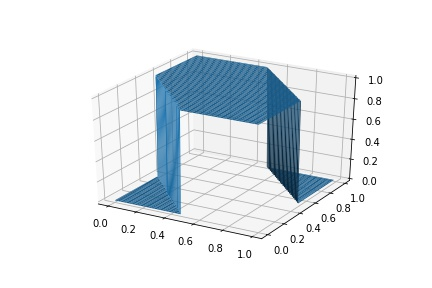
\includegraphics[width=10cm]{./images/exercise2.5.jpg}
    \caption{Exercise2.5の出力結果}
    \label{fig:exercise2.5}
  \end{figure}

  \paragraph{ 考察}
  本課題では,ステップ関数を用いたニューラルネットワークの出力をグラフ化して表示した.その事によりweightの値によってどうやって出力が変化しているのか視覚化されてわかりやすくなった.

  %%%%%%%%%%%%%%%%%%%%%%%%%%%%%%%%%%%%%%%%%%%%%%%%%%%%%%%%%%%%%%%%%%%%%%%%%%%%%
  % Exercise 2.6
  %%%%%%%%%%%%%%%%%%%%%%%%%%%%%%%%%%%%%%%%%%%%%%%%%%%%%%%%%%%%%%%%%%%%%%%%%%%%%
  \subparagraph{Exercise~2.6}
  \paragraph{ 課題内容}
  If we slightly change the value of weights or biases in exercise2\_4.m, please check how the output value changes.

  \paragraph{ 解答}
  もしweightsとbiasesの値を少し変えたら出力はどうなるのか確認せよという課題だった.ソースコードの一部とその出力結果を以下に示す.

  \begin{lstlisting}[caption=Exercise~2.6, label=src:exercise2.6]
x = np.array([[0,0,1,1],
              [0,1,0,1]])
w = np.array([[1.5, 0.5],
              [-0.5, -1.1]])
b = np.array([[0],
              [1]])
u = np.array([0.5, 1.5])
c = np.array([-2])

layer1 = Affine(w,b)
layer2 = Sigmoid()
layer3 = Affine(u,c)
layer4 = Sigmoid()

p = layer1.forward(x)
y = layer2.forward(p)
q = layer3.forward(y)
z = layer4.forward(q)
print(y)
print(z)
  \end{lstlisting}

  \begin{itembox}[l]{出力結果}
    \begin{verbatim}
[[0.5        0.62245933 0.81757448 0.88079708]
 [0.73105858 0.47502081 0.62245933 0.35434369]]
[0.34222103 0.27363866 0.34129608 0.26345536]
    \end{verbatim}
  \end{itembox}

  \paragraph{ 考察}
  本課題では,weightsやbiasesを少し変えると出力も少しだけ変わるということが分かった.これにより,ニューラルネットの保持する状態(weightやbias)を少しづつ変化させると出力も少しづつ変えることができるということが分かった.

  %%%%%%%%%%%%%%%%%%%%%%%%%%%%%%%%%%%%%%%%%%%%%%%%%%%%%%%%%%%%%%%%%%%%%%%%%%%%%
  % Chapter 3
  % Exercise 3.4
  %%%%%%%%%%%%%%%%%%%%%%%%%%%%%%%%%%%%%%%%%%%%%%%%%%%%%%%%%%%%%%%%%%%%%%%%%%%%%
  \section{Chapter~3}
  \subsection{Exercise~3.4}
  \paragraph{ 課題内容}
  Check the values of output y, layer1.weights and layer1.bias after learning in example3\_2.m.

  \paragraph{ 解答}
  課題は学習のプログラムを実行した後のレイヤ1のweightとbiasを確認せよという課題だった.ソースコードの一部とその出力結果を以下に示す.

  \begin{lstlisting}[caption=Exercise~3.4, label=src:exercise3.4]
class Affine:
    def __init__(self, w, b):
        self.w = w
        self.b = b
        self.dw = None
        self.db = None
        self.input = None

    def forward(self, x):
        self.input = x
        y = np.dot(self.w, x) + self.b
        return y

    def backward(self, dx):
        self.dw = np.dot(dx ,self.input.T)
        self.db = np.sum(dx, axis=1, keepdims=True)
        return np.dot(self.w.T, dx)

    def update(self, lr=0.1):
        self.w -= self.dw * lr
        self.b -= self.db * lr

class Sigmoid:
    def __init__(self):
        self.output = None

    def forward(self, x):
        y = 1 / (1 + np.exp(-x))
        self.output = y
        return y

    def backward(self, dx):
        return dx * self.output * (1.0 - self.output)


x = np.array([[0, 0, 1, 1],
              [0, 1, 0, 1]])
t = np.array([0, 0, 0, 1])

input_dim = 2
hidden_dim = 2
output_dim = 1

w = 2.0 * np.random.rand(1, 2) - 1.0
b = 2.0 * np.random.rand(1, 1) - 1.0

layer1 = Affine(w, b)
layer2 = Sigmoid()
layer3 = MSE()

epoch = 1000
for i in range(epoch):
    p = layer1.forward(x)
    y = layer2.forward(p)
    loss = layer3.forward(y, t)

    dy = layer3.backward()
    dp = layer2.backward(dy)
    dx = layer1.backward(dp)

    layer1.update()

    if i % 100 == 0:
        print('epoch', i, 'loss', loss, 'y', y)

print(layer1.w)
print(layer1.b)
  \end{lstlisting}

  \begin{itembox}[l]{出力結果}
    {\footnotesize
    \begin{verbatim}
epoch 0 loss 0.11059875819525353 y [[0.30140249 0.16058501 0.36526844 0.20329552]]
epoch 100 loss 0.07264510880272602 y [[0.22688731 0.27025334 0.39495912 0.45168125]]
epoch 200 loss 0.0527648595295762 y [[0.14751532 0.29044564 0.34971152 0.55988491]]
epoch 300 loss 0.0417154667463111 y [[0.09939268 0.28169867 0.30972685 0.61456522]]
epoch 400 loss 0.03449939597385088 y [[0.07045038 0.26694585 0.28070435 0.65218267]]
epoch 500 loss 0.029323894473012743 y [[0.05202754 0.25143319 0.25849141 0.68086392]]
epoch 600 loss 0.025403024800220022 y [[0.03971709 0.23684354 0.24062763 0.70394218]]
epoch 700 loss 0.022326384745484495 y [[0.03115796 0.22363927 0.22575441 0.72312334]]
epoch 800 loss 0.019851247873327545 y [[0.02500759 0.21184582 0.21307449 0.73941371]]
epoch 900 loss 0.017821589787150982 y [[0.02046322 0.20134291 0.20208214 0.75346842]]
[[2.62166652 2.61870924]]
[[-4.05594338]]
    \end{verbatim}}
  \end{itembox}

  \paragraph{ 考察}
  本課題ではAND回路の入力と出力を使ってニューラルネットワークを学習させた.そして実行したあとのレイヤ1のウェイトとバイアスとそれらを使った出力を表示させた.しかし,結果を見たところ学習しきっているようには見えなかった.ただ,損失関数の値の下がり具合を見ると,学習途中のように見えたのでエポックを増やせばまだ損失は下がりそうだと感じた.

  %%%%%%%%%%%%%%%%%%%%%%%%%%%%%%%%%%%%%%%%%%%%%%%%%%%%%%%%%%%%%%%%%%%%%%%%%%%%%
  % Exercise 3.5
  %%%%%%%%%%%%%%%%%%%%%%%%%%%%%%%%%%%%%%%%%%%%%%%%%%%%%%%%%%%%%%%%%%%%%%%%%%%%%
  \subsection{Exercise~3.5}
  \paragraph{ 課題内容}
  Check the values of weights and biases after learning in example3\_3.m and write down these values to one places of decimals. Then, calculate XOR output by your hand calculation with step function.

  \paragraph{ 解答}
  課題内容はXORの入力と出力を使ってニューラルネットを学習させ,各レイヤのウェイトとバイアスを表示させ手作業で計算もするということだった.ソースコードと出力結果,手作業で計算した結果を以下に示す.

  \begin{lstlisting}[caption=Exercise~3.5, label=src:exercise3.5]
x = np.array([[0, 0, 1, 1],
              [0, 1, 0, 1]])
t = np.array([0, 1, 1, 0])

input_dim = 2
hidden_dim = 2
output_dim = 1

w = 2.0 * np.random.rand(hidden_dim, input_dim) - 1.0
b = 2.0 * np.random.rand(hidden_dim, 1) - 1.0
u = 2.0 * np.random.rand(output_dim, hidden_dim) -1.0
c = 2.0 * np.random.rand(output_dim, 1) - 1.0

layer1 = Affine(w, b)
layer2 = Sigmoid()
layer3 = Affine(u, c)
layer4 = Sigmoid()
layer5 = MSE()

epoch = 1000
for i in range(epoch):
    p = layer1.forward(x)
    y = layer2.forward(p)
    q = layer3.forward(y)
    z = layer4.forward(q)
    loss = layer5.forward(z, t)

    dz = layer5.backward()
    dq = layer4.backward(dz)
    dy = layer3.backward(dq)
    dp = layer2.backward(dy)
    dx = layer1.backward(dp)

    layer1.update(1.0)
    layer3.update(1.0)

    if i % 100 == 0:
        print('epoch', i, 'loss', loss, 'z', z)
  \end{lstlisting}

  \begin{itembox}[l]{出力結果}
    {\footnotesize
    \begin{verbatim}
epoch 0 loss 0.14865152481975835 z [[0.30973394 0.29240501 0.27691086 0.26406156]]
epoch 100 loss 0.12493005821637666 z [[0.51293776 0.50855688 0.49162716 0.4861852 ]]
epoch 200 loss 0.12465843369022318 z [[0.51062719 0.51422939 0.48651222 0.48670789]]
epoch 300 loss 0.12365131549983245 z [[0.51059522 0.53086825 0.47145759 0.47860356]]
epoch 400 loss 0.11606619291149047 z [[0.49631644 0.6006541  0.42374649 0.43663975]]
epoch 500 loss 0.0929762025847744 z [[0.45748439 0.74956163 0.39729043 0.32945326]]
epoch 600 loss 0.04646288191252964 z [[0.35850376 0.79248915 0.60704202 0.21377882]]
epoch 700 loss 0.009311833893073414 z [[0.14334216 0.86844748 0.8509094  0.12005676]]
epoch 800 loss 0.004461025559716306 z [[0.09645524 0.90192461 0.90219031 0.08484735]]
epoch 900 loss 0.0028436916336632635 z [[0.07621343 0.91943909 0.92374011 0.06808389]]
[[ 4.22786955 -4.5941637 ]
 [ 5.50647153 -5.78792623]]
[[-2.25110444]
 [ 3.17054042]]
[[ 7.18034835 -6.66447265]]
[[3.03835718]]
    \end{verbatim}}
  \end{itembox}

  1000エポック分学習させた状態で出力を手計算でステップ関数を適用させると,
  \begin{equation*}
    \begin{bmatrix}0.1&0.9&0.9&0.1\end{bmatrix} = \begin{bmatrix}0&1&1&0\end{bmatrix} \qquad (\text{ステップ関数適用})
  \end{equation*}

  \paragraph{ 考察}
  本課題でXORの入力と出力を学習させて,その出力を手計算でステップ関数を適用させた.まず,前提として資料に載っていた学習設定では学習しきっていなさそうだったため,学習率を0.1から1.0まで引き上げた.そうしたら500エポックを超え始めたあたりから急激に損失関数の出力が下がりはじめた様に見えた.また,実際に手作業でステップ関数も適用させた結果から正しく学習できているということが分かった.

  %%%%%%%%%%%%%%%%%%%%%%%%%%%%%%%%%%%%%%%%%%%%%%%%%%%%%%%%%%%%%%%%%%%%%%%%%%%%%
  % Chapter 4
  % Exercise 4.3
  %%%%%%%%%%%%%%%%%%%%%%%%%%%%%%%%%%%%%%%%%%%%%%%%%%%%%%%%%%%%%%%%%%%%%%%%%%%%%
  \section{Chapter~4}
  \subsection{Exercise~4.3}
  \paragraph{ 課題内容}
  Try to increase the performance of the neural network by setting the parameter to various values. Consider the recognition accuracy, parameter values such as the number of hidden layer neurons, learning rate, epoch number and initial weights and biases, and what kind of images are difficult to recognize, and put the consideration and findings together in your final report.

  \paragraph{ 解答}
  課題内容がExercise4.2で学習させた結果より精度を上げるためにハイパーパラメータなどを変更せよとのことだった.まずはExercise4.2の出力を以下に示す.

  \begin{itembox}[l]{出力結果}
    {\footnotesize
    \begin{verbatim}
epoch:0 loss:0.3379676518566211
epoch:1 loss:0.23594588128504435
epoch:2 loss:0.1722073375253008
epoch:3 loss:0.13766380775297515
epoch:4 loss:0.1176365801136934

[[5523    2   83   18   19  120   73   29   53    3]
 [   4 6489   45   37   12   27   12   18   83   15]
 [ 107   85 4932  140  144   24  196  116  183   31]
 [ 101   79  157 5163   15  307   33   71  139   66]
 [   6   45   69    7 5250   11  121   17   25  291]
 [ 208   61   54  305   75 4121  151   49  319   78]
 [  84   40   86    6   49  151 5418    8   72    4]
 [  29   90   74   80  123   21   10 5516   28  294]
 [  21  166  124  243   83  376   59   34 4620  125]
 [  28   39   36   69  281   53    8  214   93 5128]]
train_accuary=0.8693333333333333

[[ 940    0    2    3    1   13    9    5    6    1]
 [   0 1102    5    4    1    2    5    1   14    1]
 [  17   12  859   20   22    2   27   24   38   11]
 [  13   14   32  848    4   49    2   11   27   10]
 [   2    3    4    1  885    1   29    0    2   55]
 [  26    8    5   58   12  681   18   16   54   14]
 [  17    7    6    2    9   29  874    5    6    3]
 [  10   21   26   11   15    1    1  888    0   55]
 [   5   19   14   30   17   58   10   11  783   27]
 [   2    6    3    9   38   13    4   17   10  907]]
test_accuary=0.8767
    \end{verbatim}}
  \end{itembox}

  \begin{figure}[h]
    \centering
    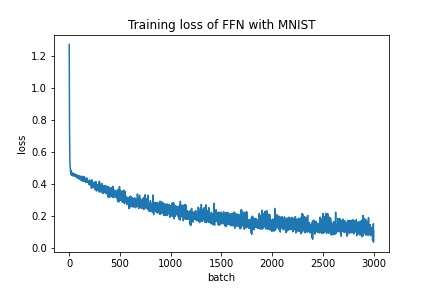
\includegraphics[width=10cm]{images/exercise4.2.jpg}
    \caption{MNISTデータにおけるFFNモデル学習時の損失関数}
    \label{fig:mnist-ffn-loss}
  \end{figure}

  以上の結果から精度を上げるためにハイパーパラメータを変更した.具体的にはエポックを5から20,中間層の次元数を10から50に変更すると以下のような結果が得られた.また,そのソースコードも以下に示す.

 \begin{lstlisting}[basicstyle=\small, caption=Exercise~3.5, label=src:exercise3.5]
class Dataset:
    def __init__(self, data_dir=None, data=None, transform=None, train=True):
        self.data_dir = data_dir
        self.transform = transform
        self.train = train

    def __getitem__(self, idx):
        raise NotImplementedError


class MNISTDataset(Dataset):

    urls = [
        'http://yann.lecun.com/exdb/mnist/train-images-idx3-ubyte.gz',
        'http://yann.lecun.com/exdb/mnist/train-labels-idx1-ubyte.gz',
        'http://yann.lecun.com/exdb/mnist/t10k-images-idx3-ubyte.gz',
        'http://yann.lecun.com/exdb/mnist/t10k-labels-idx1-ubyte.gz',
    ]

    def __init__(self, data_dir, transform=None, train=True):
        super(MNISTDataset, self).__init__(data_dir,
                                           transform=transform,
                                           train=train)

        if not self._exist_data():
            print('Start downloading MNIST data from http://yann.lecun.com/exdb/mnist/')
            self.download()
            print('Complete!')

        if self.train:
            self.data = (
                read_mnist_data(os.path.join(self.data_dir, 'train-images-idx3-ubyte.gz')),
                read_mnist_data(os.path.join(self.data_dir, 'train-labels-idx1-ubyte.gz')),
            )
        else:
            self.data = (
                read_mnist_data(os.path.join(self.data_dir, 't10k-images-idx3-ubyte.gz')),
                read_mnist_data(os.path.join(self.data_dir, 't10k-labels-idx1-ubyte.gz')),
            )

    def __getitem__(self, idx):
        images = self.data[0][idx]
        labels = self.data[1][idx]

        if self.transform:
            images, labels = self.transform((images, labels))

        return images, labels

    def __len__(self):
        return self.data[0].shape[0]

    def download(self):
        import urllib.request

        os.makedirs(self.data_dir, exist_ok=True)

        for url in self.urls:
            filename = url.rpartition('/')[2]
            urllib.request.urlretrieve(url, os.path.join(self.data_dir, filename))

        return

    def _exist_data(self):
        for url in self.urls:
            filename = url.rpartition('/')[2]
            if not os.path.isfile(os.path.join(self.data_dir, filename)):
                return False

        return True


class DataLoader:
    def __init__(self, dataset, batch_size=100):
        self.dataset = dataset
        self._batch_size = batch_size
        self._i = 0

    def __iter__(self):
        return self

    def __next__(self):
        if (self._i * self._batch_size) >= len(self.dataset):
            self._i = 0
            raise StopIteration
        elif ((self._i + 1) * self._batch_size) >= len(self.dataset):
            x, y = self.dataset[self._i * self._batch_size:]
        else:
            x, y = self.dataset[self._i * self._batch_size:(self._i + 1) * self._batch_size]

        self._i += 1
        return x, y


def read_mnist_data(filepath):
    import gzip, codecs
    with gzip.open(filepath, 'rb') as f:
        data = f.read()

    magic = int(codecs.encode(data[0:4], 'hex'), 16)
    nd = magic % 256
    ty = magic // 256
    data_num = int(codecs.encode(data[4:8], 'hex'), 16)

    return np.frombuffer(data, dtype=np.uint8, offset=(4 * (nd + 1))).reshape(data_num, -1)


class MNISTTransform:
    def __init__(self):
        pass

    def __call__(self, data):
        x = data[0] / 255
        y = np.identity(10)[data[1].flatten()]

        return (x, y)

epochs = 20  # 5 -> 20へ変更
batch_size = 100
input_dim = 784
hidden_dim = 50 # 10 -> 50へ変更
output_dim = 10

mnist_train = MNISTDataset('../data/mnist', transform=MNISTTransform(), train=True)
mnist_test = MNISTDataset('../data/mnist', transform=MNISTTransform(), train=False)
dataloader_train = DataLoader(mnist_train, batch_size=batch_size)
dataloader_test = DataLoader(mnist_test, batch_size=batch_size)

w = np.random.randn(hidden_dim, input_dim)
b = np.random.randn(hidden_dim, 1)
u = np.random.randn(output_dim, hidden_dim)
c = np.random.randn(output_dim, 1)

layer1 = Affine(w, b)
layer2 = Sigmoid()
layer3 = Affine(u, c)
layer4 = Sigmoid()
layer5 = MSE()

loss = []

for epoch in range(epochs):
    predicts = []
    for x, y in dataloader_train:
        p = layer1.forward(x.T)
        t = layer2.forward(p)
        q = layer3.forward(t)
        z = layer4.forward(q)
        predicts.append(list(z.T))
        loss.append(layer5.forward(z, y.T))

        dz = layer5.backward()
        dq = layer4.backward(dz)
        dt = layer3.backward(dq)
        dp = layer2.backward(dt)
        dx = layer1.backward(dp)

        layer1.update(lr=0.05)
        layer3.update(lr=0.05)
    print('epoch:{epoch} loss:{loss}'.format(epoch=epoch, loss=loss[-1]))

images, labels = mnist_train[0:]
predicts = np.identity(10)[np.argmax(np.array(predicts).reshape(-1, 10), axis=1)]
results = np.dot(labels.T, predicts).astype(np.int32)

print(results)
print('accuary={}'.format(np.diag(results).sum() / results.sum()))

plt.plot(np.arange(12000), np.array(loss))
plt.title('Training loss of FFN with MNIST')
plt.xlabel('batch')
plt.ylabel('loss')
plt.show()

predicts = []

for x, y in dataloader_test:
    p = layer1.forward(x.T)
    y = layer2.forward(p)
    q = layer3.forward(y)
    z = layer4.forward(q)
    predicts.append(list(z.T))

images, labels = mnist_test[0:]
predicts = np.identity(10)[np.argmax(np.array(predicts).reshape(-1, 10), axis=1)]
results = np.dot(labels.T, predicts).astype(np.int32)

print(results)
print('accuary={}'.format(np.diag(results).sum() / results.sum()))
  \end{lstlisting}

  \begin{itembox}[l]{出力結果}
    {\footnotesize
    \begin{verbatim}
epoch:0 loss:0.2523595456655897
epoch:1 loss:0.1783767324616495
epoch:2 loss:0.13051501818352595
epoch:3 loss:0.11571855536826176
epoch:4 loss:0.08457559114881316
epoch:5 loss:0.05905629578978815
epoch:6 loss:0.051956685309520426
epoch:7 loss:0.047524731738717844
epoch:8 loss:0.04473252626393911
epoch:9 loss:0.04225189062581892
epoch:10 loss:0.03969878490015143
epoch:11 loss:0.037133564395709875
epoch:12 loss:0.03470599079638301
epoch:13 loss:0.03251194227002699
epoch:14 loss:0.030504217377877056
epoch:15 loss:0.028733949273416725
epoch:16 loss:0.02733138361801906
epoch:17 loss:0.026216503928003555
epoch:18 loss:0.025227079373516093
epoch:19 loss:0.024355322842522995

[[5799    1    9    3    9   17   29    9   42    5]
 [   3 6616   30   23    7    7    7   15   24   10]
 [  27   18 5635   44   51   10   40   49   71   13]
 [  16   16   99 5700    7   92   15   61   89   36]
 [  11   20   20    2 5591    4   28   16   12  138]
 [  32   12   27   79   26 5093   42   21   50   39]
 [  36    6   10    0   29   48 5759    2   25    3]
 [  11   26   47   15   41    3    3 6034   16   69]
 [  24   44   38   74   16   52   25   17 5519   42]
 [  33    9    9   59  102   21   10   82   52 5572]]
accuary=0.9553

[[ 959    0    0    2    2    4    6    3    4    0]
 [   0 1118    3    2    1    2    3    1    5    0]
 [   5    2  951   14   13    4    8   15   18    2]
 [   0    1   10  942    1   16    0   10   22    8]
 [   2    1    3    1  928    0    7    1    3   36]
 [   6    1    0   21    4  823    9    2   18    8]
 [  12    3    5    0    7   12  911    1    7    0]
 [   1    8   20    5    6    1    0  964    2   21]
 [   5    3    3   13   10   17    8    9  894   12]
 [   6    6    1    6   24   14    3    8    5  936]]
accuary=0.9426
    \end{verbatim}}
  \end{itembox}

  \newpage

  \begin{figure}[h]
    \centering
    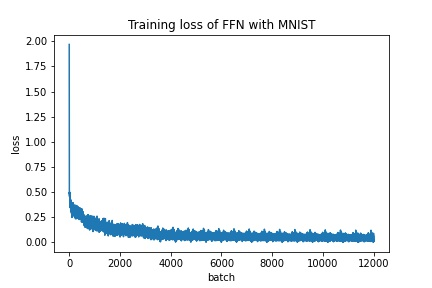
\includegraphics[width=10cm]{images/exercise4.3.jpg}
    \caption{ハイパーパラメータを変更した後のモデル学習時の損失関数}
    \label{fig:mnist-ffn-tuned-loss}
  \end{figure}

  \paragraph{ 考察}
  まず,前課題で学習させたモデルのtrain, testの各精度は86.93\%と87.67\%となっていた.そこからハイパーパラメータのエポック数と中間層の次元数をそれぞれ5から20,10から50というふうに変えて再度モデルを学習させた.そうしたらtrain,testの各精度は95.53\%,94.26\%と約10\%近くも向上した.エポック数を増やすと学習がより進み,中間層の次元を増やすとより柔軟なモデルにすることができ,モデルの表現力が上がる.その双方の効果が出て10\%近くも精度が向上したのではないかと考えた.


\end{document}
